% Options for packages loaded elsewhere
\PassOptionsToPackage{unicode}{hyperref}
\PassOptionsToPackage{hyphens}{url}
\PassOptionsToPackage{dvipsnames,svgnames,x11names}{xcolor}
%
\documentclass[
  authoryear,
  preprint,
  3p]{elsarticle}

\usepackage{amsmath,amssymb}
\usepackage{iftex}
\ifPDFTeX
  \usepackage[T1]{fontenc}
  \usepackage[utf8]{inputenc}
  \usepackage{textcomp} % provide euro and other symbols
\else % if luatex or xetex
  \usepackage{unicode-math}
  \defaultfontfeatures{Scale=MatchLowercase}
  \defaultfontfeatures[\rmfamily]{Ligatures=TeX,Scale=1}
\fi
\usepackage{lmodern}
\ifPDFTeX\else  
    % xetex/luatex font selection
\fi
% Use upquote if available, for straight quotes in verbatim environments
\IfFileExists{upquote.sty}{\usepackage{upquote}}{}
\IfFileExists{microtype.sty}{% use microtype if available
  \usepackage[]{microtype}
  \UseMicrotypeSet[protrusion]{basicmath} % disable protrusion for tt fonts
}{}
\makeatletter
\@ifundefined{KOMAClassName}{% if non-KOMA class
  \IfFileExists{parskip.sty}{%
    \usepackage{parskip}
  }{% else
    \setlength{\parindent}{0pt}
    \setlength{\parskip}{6pt plus 2pt minus 1pt}}
}{% if KOMA class
  \KOMAoptions{parskip=half}}
\makeatother
\usepackage{xcolor}
\setlength{\emergencystretch}{3em} % prevent overfull lines
\setcounter{secnumdepth}{5}
% Make \paragraph and \subparagraph free-standing
\ifx\paragraph\undefined\else
  \let\oldparagraph\paragraph
  \renewcommand{\paragraph}[1]{\oldparagraph{#1}\mbox{}}
\fi
\ifx\subparagraph\undefined\else
  \let\oldsubparagraph\subparagraph
  \renewcommand{\subparagraph}[1]{\oldsubparagraph{#1}\mbox{}}
\fi


\providecommand{\tightlist}{%
  \setlength{\itemsep}{0pt}\setlength{\parskip}{0pt}}\usepackage{longtable,booktabs,array}
\usepackage{calc} % for calculating minipage widths
% Correct order of tables after \paragraph or \subparagraph
\usepackage{etoolbox}
\makeatletter
\patchcmd\longtable{\par}{\if@noskipsec\mbox{}\fi\par}{}{}
\makeatother
% Allow footnotes in longtable head/foot
\IfFileExists{footnotehyper.sty}{\usepackage{footnotehyper}}{\usepackage{footnote}}
\makesavenoteenv{longtable}
\usepackage{graphicx}
\makeatletter
\def\maxwidth{\ifdim\Gin@nat@width>\linewidth\linewidth\else\Gin@nat@width\fi}
\def\maxheight{\ifdim\Gin@nat@height>\textheight\textheight\else\Gin@nat@height\fi}
\makeatother
% Scale images if necessary, so that they will not overflow the page
% margins by default, and it is still possible to overwrite the defaults
% using explicit options in \includegraphics[width, height, ...]{}
\setkeys{Gin}{width=\maxwidth,height=\maxheight,keepaspectratio}
% Set default figure placement to htbp
\makeatletter
\def\fps@figure{htbp}
\makeatother

\usepackage{booktabs}
\usepackage{longtable}
\usepackage{array}
\usepackage{multirow}
\usepackage{wrapfig}
\usepackage{float}
\usepackage{colortbl}
\usepackage{pdflscape}
\usepackage{tabu}
\usepackage{threeparttable}
\usepackage{threeparttablex}
\usepackage[normalem]{ulem}
\usepackage{makecell}
\usepackage{xcolor}
\usepackage{todonotes,mathtools,bm,amsmath,mathpazo,xcolor}
\mathtoolsset{showonlyrefs}
\setlength{\parindent}{0cm}
\usepackage{tikz}
\usetikzlibrary{positioning, shapes.geometric, arrows.meta, fit}
\tikzset{
  process/.style={
  rectangle,
  draw=black,
  thick,
  text width=4.5cm,
  align=center,
  minimum height=1.4cm
  },
groupbox/.style={
  draw=black,
  thick,
  dashed,
  inner sep=0.3cm,
  rounded corners,
  label={[black]90:#1}
},
arrow/.style={
  thick,
  ->,
  >=Stealth
}
        }
\makeatletter
\@ifpackageloaded{caption}{}{\usepackage{caption}}
\AtBeginDocument{%
\ifdefined\contentsname
  \renewcommand*\contentsname{Table of contents}
\else
  \newcommand\contentsname{Table of contents}
\fi
\ifdefined\listfigurename
  \renewcommand*\listfigurename{List of Figures}
\else
  \newcommand\listfigurename{List of Figures}
\fi
\ifdefined\listtablename
  \renewcommand*\listtablename{List of Tables}
\else
  \newcommand\listtablename{List of Tables}
\fi
\ifdefined\figurename
  \renewcommand*\figurename{Figure}
\else
  \newcommand\figurename{Figure}
\fi
\ifdefined\tablename
  \renewcommand*\tablename{Table}
\else
  \newcommand\tablename{Table}
\fi
}
\@ifpackageloaded{float}{}{\usepackage{float}}
\floatstyle{ruled}
\@ifundefined{c@chapter}{\newfloat{codelisting}{h}{lop}}{\newfloat{codelisting}{h}{lop}[chapter]}
\floatname{codelisting}{Listing}
\newcommand*\listoflistings{\listof{codelisting}{List of Listings}}
\makeatother
\makeatletter
\makeatother
\makeatletter
\@ifpackageloaded{caption}{}{\usepackage{caption}}
\@ifpackageloaded{subcaption}{}{\usepackage{subcaption}}
\makeatother
\journal{International Journal of Production Research}
\ifLuaTeX
  \usepackage{selnolig}  % disable illegal ligatures
\fi
\usepackage[]{natbib}
\bibliographystyle{elsarticle-harv}
\usepackage{bookmark}

\IfFileExists{xurl.sty}{\usepackage{xurl}}{} % add URL line breaks if available
\urlstyle{same} % disable monospaced font for URLs
\hypersetup{
  pdftitle={The missing puzzle piece: contextual insights for enhanced pharmaceutical supply chain forecasting},
  pdfauthor={Arebu Issa Bilal; Bahman Rostami-Tabar; Harsha Halgamuwe Hewage; Umit Sezer Bititci; Teferi Gedif Fenta},
  pdfkeywords={Forecasting, Pharmaceutical supply chain, Domain
knowlege, Forecast accuracy, Developing countries},
  colorlinks=true,
  linkcolor={blue},
  filecolor={Maroon},
  citecolor={Blue},
  urlcolor={Blue},
  pdfcreator={LaTeX via pandoc}}

\setlength{\parindent}{6pt}
\begin{document}

\begin{frontmatter}
\title{The missing puzzle piece: contextual insights for enhanced
pharmaceutical supply chain forecasting}
\author[1]{Arebu Issa Bilal%
\corref{cor1}%
}
 \ead{arebu.issa@aau.edu.et} 
\author[2]{Bahman Rostami-Tabar%
%
}
 \ead{rostami-tabarb@cardiff.ac.uk} 
\author[2]{Harsha Halgamuwe Hewage%
%
}
 \ead{HalgamuweHewageHR@cardiff.ac.uk} 
\author[3]{Umit Sezer Bititci%
%
}
 \ead{U.S.Bititci@hw.ac.uk} 
\author[1]{Teferi Gedif Fenta%
%
}
 \ead{tgedif@gmail.com} 

\affiliation[1]{organization={Addis Ababa University, Department of
Social and Administrative Pharmacy, School of
Pharmacy},country={Ethiopia.},countrysep={,},postcodesep={}}
\affiliation[2]{organization={Cardiff University, Data Lab for Social
Good Research Group, Cardiff Business
School},country={UK.},countrysep={,},postcodesep={}}
\affiliation[3]{organization={Heriot-Watt University, Edinburgh Business
School, Heriot-Watt
University},country={UK.},countrysep={,},postcodesep={}}

\cortext[cor1]{Corresponding author}





        
\begin{abstract}
Accurate forecasting in pharmaceutical supply chains is critical for
ensuring the continuous availability of essential medicines,
particularly in developing countries where resource constraints and
logistical challenges are more pronounced. Effective demand forecasting
supports procurement and inventory management, which in turn could help
to prevent stockouts, reduce wastage due to overstocking, and enhance
overall healthcare delivery. In such settings, reliable forecasts that
acknowledge uncertainties, are essential to ensure that limited
resources are used efficiently to meet health needs. Despite
advancements in forecasting, significant gaps remain in effective
forecasting in poor resource countries. Most existing literature on
pharmaceutical supply chain forecasting focuses primarily on point
estimation while neglecting the inherent uncertainty of these forecasts.
Additionally, these studies often rely solely on historical consumption
and distribution data, overlooking the broader contextual factors that
shape these patterns. Furthermore, many works lack rigorous
methodological design, transparency, and reproducibility. This study
addresses these gaps by integrating domain-specific knowledge, gathered
through expert interviews and engagement with key members of the
Ethiopian Pharmaceutical Supply Service, into forecasting models. Using
a dataset spanning five years (December 2017 to July 2022) from EPSS, we
developed forecasting models that integrate expert-identified variables
such as stock replenishment schedules, fiscal inventory counts, and
disease outbreaks. Evaluation metrics including Mean Absolute Scaled
Error, Root Mean Squared Scaled Error, and Continuous Ranked Probability
Score are used to report forecast accuracy. The findings underscore the
significance of contextual data in developing robust forecasting models
that are adaptable to complex, real-world conditions. Our results also
highlight the effectiveness of foundational time series models for
forecasting. These models are particularly appealing for
resource-constrained countries that may lack advanced analytical
expertise. To promote usability, generalizability, and reproducibility,
we share the complete dataset and code in R and Python, and the entire
paper is written in Quarto via a GitHub repository to facilitate these
practices.
\end{abstract}





\begin{keyword}
    Forecasting \sep Pharmaceutical supply chain \sep Domain
knowlege \sep Forecast accuracy \sep 
    Developing countries
\end{keyword}
\end{frontmatter}
    
\section{Introduction}\label{sec-intro}

Universal access to essential medicines is a fundamental goal of
effective healthcare systems, yet ensuring equitable availability
continues to be a critical global challenge
\citep{quick2003essential, world2004annual}. Many countries,
particularly in Africa and Asia, face significant barriers to accessing
these medications, often due to high costs and inefficient supply chain
management \citep{world2004medicines}. A survey conducted in eight
sub-Saharan African countries revealed alarmingly low availability of
essential medicines. The average availability of women's priority
medicines ranged from just 22\% to 40\%, while children's medicines were
only slightly more accessible, with availability ranging from 28\% to
57\% \citep{droti2019poor}. However, drug shortages are not limited to
low-income regions; they also occur in developed areas like the United
States and Europe, where they disrupt healthcare delivery and compromise
the quality of patient care
\citep{fox2003managing, kaakeh2011impact, johnson2011drug, huys2013european, le2011prevalence}.

The consequences of drug shortages extend beyond immediate healthcare
delivery, impacting healthcare costs, treatment quality, and patient
safety \citep{alspach2012drug, kaakeh2011impact, baumer2004national}.
Such shortages can result in treatment delays, suboptimal care due to
the unavailability of preferred therapies, increased reliance on costly
secondary markets, and serious patient outcomes, including
complications, longer hospital stays, and even deaths
\citep{alspach2012drug}. Addressing these challenges requires a
resilient pharmaceutical supply chain that can ensure the timely
availability of medicines. In this context, accurate demand forecasting
becomes critical for effective procurement and inventory management
\citep{subramanian2021effective}.

Demand forecasting in pharmaceutical supply chains is a highly complex
process, shaped by several factors. These include the quality of
available data, the specific position within the supply chain, and
external influences such as market trends, regulatory changes, and
disruptive events such as pandemics, conflicts, flooding
\citep{schneider2010pharmaceutical, hyndman2018forecasting}. Recently,
major donors such as Bill \& Melinda Gates Foundation have invested in
data collection technologies in sub-Saharan Africa, recognizing the
potential of data to provide valuable insights. This investment is
essential and offers significant benefits for improving supply chain
delivery. However, much of the data being collected focuses on
transactional data, such as consumption, distribution, and sale. Almost
all platforms collecting data tend to overlook the critical contextual
factors and events that influence these transactions---factors that are
just as crucial for accurate forecasting. This presents a major barrier,
as understanding the broader context, including administration
procedures, local policies, disruptions, conflicts, and so on is vital
for building reliable forecasting models. This gap --- known as business
context and domain knowledge --- requires urgent attention in
pharmaceutical supply chain forecasting. Without incorporating this
knowledge, any forecasting model is unlikely to produce reliable
results. We must prioritize collecting and integrating this contextual
information to improve the accuracy of demand forecasts in
pharmaceutical supply chains. Integrating statistical models with domain
knowledge leads to a more accurate and context-aware forecasting
process, as evidenced by research that highlights the value of
judgmental adjustments to enhance forecast accuracy
\citep{fildes2007against, taylor2022artificial, soyiri2013overview}.
Domain knowledge enables analysts to incorporate relevant events, such
as supply chain disruptions, into the forecasting model. This
integration is particularly beneficial in fields like healthcare, where
expert insights can align algorithms with real-world applications
\citep{dash2022review}.

This study aims to bridge that gap by employing advanced machine
learning models combined with domain expertise to address the
distinctive characteristics of Ethiopia's pharmaceutical sector. The
challenges in this sector, such as diverse product categories, limited
data from service delivery points, communication issues, long lead
times, forecast inaccuracies, and complex policies, necessitate tailored
forecasting approaches
\citep{bilal2024challenges, boche2022procurement}. Accurate demand
forecasting in Ethiopia is essential for optimizing resource allocation,
streamlining supply chain operations, and shaping effective healthcare
policies \citep{rostami2022forecasting}.

This research uses distribution data from 33 health commodities,
covering the period from December 2017 to July 2022, provided by the
Ethiopian Pharmaceutical Supply Service (EPSS), to develop models for
six-month-ahead forecasting. Initially, we implement univariate models
that rely solely on distribution data. Following this, we conduct
exploratory data analysis and engage in interviews with EPSS experts to
gather domain knowledge on events influencing distribution patterns.
Through these interviews, the experts identified three key factors
collectively impacting distribution: stock replenishment period, fiscal
calendar, and the seasonal malaria. We then develop forecasting models
that incorporate the data gathered through the interview process and
compare their performance with univariate models that rely solely on
distribution data.

Our primary aims is to assess whether incorporating domain knowledge
improves forecast accuracy. Moreover, we also fill a gap in the
pharmaceutical demand forecasting literature by not only generating
point forecasts but also producing probabilistic forecasting techniques
that capture the range of potential outcomes with associated
probabilities, offering a more comprehensive view of demand uncertainty
than traditional methods. Model performance is evaluated using point
accuracy measure including MASE, RMSSE, and probabilistic measure using
CRPS.

The remainder of this paper is structured as follows: Section 2 reviews
the literature and identifies gaps to position our work; Section 3
outlines the experimental design, including data sources, forecasting
methods, and evaluation criteria; Section 4 presents the results and
analysis; and Section 5 concludes with a summary of findings and future
research directions.

\section{Research background}\label{sec-lit}

Accurate demand forecasting is crucial in the pharmaceutical industry,
where it directly impacts profit maximization, cost minimization, and
the ability to respond to market changes. Forecasting in healthcare not
only influences clinical decisions but also plays a pivotal role in
supply chain management, ensuring that the right drugs are available
when needed. The challenge lies in balancing customer demand with
inventory costs, which is particularly complex in pharmaceuticals due to
factors like short shelf life and quality constraints
\citep{gupta2000mid, makridakis2020forecasting}.

A range of methods is used in pharmaceutical supply chain forecasting,
from traditional statistical models to advanced machine learning
techniques, with many studies combining both simple and advanced
approaches to improve accuracy
\citep{nikolopoulos2016forecasting, zhu2021demand, anusha2014demand}.
Some studies, such as those by \citet{newberne2006holt}, and
\citet{restyana2021analysis}, applied traditional forecasting methods.
In contrast, other researchers explored more advanced approaches,
including hybrid models and machine learning techniques, to address
complex forecasting challenges, as seen in the studies by
\citet{siddiqui2022hybrid}, \citet{de2021lead}, \citet{kim2015demand},
\citet{candan2014demand}, and \citet{ribeiro2017improving}.

Early research in pharmaceutical forecasting primarily focused on
classical statistical methods. These methods, including ARIMA
(AutoRegressive Integrated Moving Average), exponential smoothing, and
moving averages, were widely used due to their simplicity and
effectiveness in relatively stable environments
\citep{zahra2019forecasting}. These models typically assess forecast
accuracy using metrics like Mean Absolute Percentage Error (MAPE), Mean
Squared Error (MSE), and Root Mean Squared Error (RMSE). For example,
\citet{newberne2006holt} applied the Holt-Winters method to forecast
healthcare data, focusing on prescription trends. Their findings
highlighted the method's utility in short-term planning and resource
management, validated through metrics like MAPE, MAD, and MSD.
Similarly, \citet{restyana2021analysis} compared Simple Moving Average
(SMA), and Single Exponential Smoothing (SES) in drug demand
forecasting, concluding that SES provided more accurate results, as
indicated by lower MAD and MSE values.

Recognizing the limitations of traditional models---particularly their
inability to capture the complexities of pharmaceutical demand, such as
seasonality and external influences---researchers have increasingly
turned to more advanced modeling approaches
\citep{khalil2014intelligent}. Furthermore, the growing complexity of
the pharmaceutical industry, coupled with the availability of large
datasets, has accelerated the adoption of advanced machine learning
techniques. These methods, such as Support Vector Regression (SVR),
Random Forest (RF), and Long Short-Term Memory (LSTM) networks, offer
greater flexibility and predictive power. \citet{van2021using} showed
that incorporating downstream information into machine learning models,
like LASSO and SVR, greatly enhances forecast accuracy. Their study on
multi-echelon supply chains revealed that advanced models, particularly
those integrating external variables, consistently produced lower
forecast errors, as measured by AvgRelRMSE. Similarly,
\citet{rathipriya2023demand} compared shallow neural networks and deep
learning models for drug demand forecasting. The study found that
shallow models outperformed deep learning models for most drug
categories, while ARIMA was more effective for the remaining categories.
This suggests that no single model is universally optimal, and model
selection should be context-specific.

More sophisticated models, such as Neuro-Fuzzy Systems, have emerged as
powerful tools for pharmaceutical forecasting. These systems combine the
learning capabilities of neural networks with the reasoning abilities of
fuzzy logic, offering a balanced approach that incorporates both
empirical data and expert knowledge. Deep learning models, while
powerful, present challenges such as the need for large datasets and
substantial computational resources. Despite these challenges, models
like LSTM have shown potential in capturing long-term dependencies in
time series data, as demonstrated by \citet{sousa2019statistical} in
their study on drug distribution in the Brazilian Public Health System.
\citet{candan2014demand} employed an Adaptive Neuro-Fuzzy Inference
System (ANFIS) to forecast pharmaceutical demand. Their study
highlighted the system's ability to capture complex patterns in the
data, resulting in highly accurate forecasts. The effectiveness of this
approach was further validated through statistical tests, such as paired
T-tests and mean difference analysis, which confirmed its superiority
over traditional methods.

\citet{nguyen2023managing} explore how sentiment analysis of news media
can be utilized to improve demand forecasting for pharmaceutical
products during disruptive events, such as pandemics and scandals. The
authors employed a VARX (Vector Autoregressive with Exogenous Variables)
model to forecast demand volatility. \citet{papanagnou2018coping}
investigate the impact of big data analytics, specifically through text
mining, on improving forecasting accuracy for pharmaceuticals in retail
pharmacies, using HMX pharmacy stores in Nigeria as a case study. They
use multivariate time series analysis technique known as VARX, which
incorporates customer-generated content from sources like Google,
YouTube, and online newspapers to predict demand for medicines.
\citet{fourkiotis2024applying} focus on enhancing pharmaceutical sales
forecasting through the application of both traditional statistical
methods and advanced machine learning techniques. Various forecasting
approaches, including traditional models like Naïve and ARIMA,Facebook
Prophet, and machine learning methods such as XGBoost and LSTM neural
networks are compared. The results demonstrated that machine learning
models, particularly XGBoost, significantly outperformed traditional
methods. \citet{belghith2024new} present a rolling forecasting framework
employing moving average and three exponential smoothing methods
(Brown's, Holt's, and Holt-Winters) implemented using Microsoft Power BI
for enhanced data visualization.

Table~\ref{tbl-literature} provides a summary of key studies in the
literature on forecasting for pharmaceutical products. We identify
several limitations both in the existing research and in practice, which
highlight important gaps that motivate our current study. These gaps are
summarized as follows:

\begin{enumerate}
\def\labelenumi{\arabic{enumi}.}
\item
  Despite significant investment in data collection technologies and
  logistics management systems, these systems primarily collect
  transactional data, such as consumption and distribution. However, no
  data is collected on events that influence their variability ---
  information that would be crucial for building reliable forecasting
  models. No studies to date have explored how domain expertise could
  enhance pharmaceutical demand forecasting.
\item
  Current research on forecasting for pharmaceutical supply chain
  predominantly focuses on generating point forecasts. There is a lack
  of studies that consider the entire forecast distribution, which would
  better capture the uncertainty of future demand and provide a valuable
  risk management tool for decision-makers.
\item
  Reproducibility remains a major challenge in this field. It is often
  difficult for readers to reproduce previous studies without direct
  assistance from the authors, limiting the practical application and
  validation of existing research.
\end{enumerate}

\begin{table}[H]

\caption{\label{tbl-literature}Summary of some studies on forecasting in
pharmaceutical supply chain}

\centering{

\centering\begingroup\fontsize{11}{13}\selectfont

\resizebox{\linewidth}{!}{
\begin{tabular}{lll>{\raggedright\arraybackslash}p{10em}ll>{\raggedright\arraybackslash}p{10em}>{\raggedright\arraybackslash}p{10em}>{\raggedright\arraybackslash}p{2em}>{\raggedright\arraybackslash}p{2em}>{\raggedright\arraybackslash}p{2em}}
\toprule
References & data granularity & Lenth of data & Forecast variable & Horizon & Probabilistic & Method & Metric & Items & Data & Code\\
\midrule
Current study & Monthly & 60 months & Consumption of pharmaceutical products & 6 months & Yes & TimeGpt (with and without predictors), LSTM (with and without predictors), Exponential Smoothing, ARIMA, Dynamic Regression (ARIMAX), Multiple Regression (with and without predictors) & RMSSE,CRIPS,MASE & 33 & Yes & Yes\\
Siddiqui et al. (2022) & Monthly & 58 months & Sales of pharmaceutical products & Unknown & No & ARIMA, HOLT WINTER, ETS,  Theta, ARHOW & MEAN, MAD, MSE, RMSE,  MAPE & 31 & No & No\\
de Oliveira et al.(2021) & Daily & 365 days & Lead time & NA & No & k-NN, SVM, RF, LR, MLP & MSE & 11 & Yes & No\\
Rathipriya et al. (2023) & Weekly & 260 weeks & Sales of pharmaceuticals product & Unknown & No & SNN, ARIMA P\_NN GR\_NN RBF\_NN ARIMA P\_NN GR\_NN RBF\_NN & RMSE, Normalized RMSE & 57 & Yes & No\\
Kim et al.(2015) & Monthly & 44 month & Medicines sales data & 1 month & No & VARX & Prediction error rate & 4 & No & No\\
Merkuryeva et al. (2019) & Weekly & 20 weeks & Sales of pharmaceuticals & 1–week & No & MA, Symbolic Regression, LR & R², MAD & 1 & No & No\\
Nikolopoulos et al. (2016) & Yearly & 21 year & Prescription records of pharmaceuticals & 1–5 & No & Diffusion models,  ARIMA, ES, LR & R², ME, MAE, MSE & 14 & No & No\\
Van Belle et al.(2021) & Weekly & 253 weeks & Medcine sales & 1–5 weeks & No & ARIMA, ETS, MLP, SVR, RF, LR & RMSE & 50 & No & No\\
Khalil Zadeh et al. (2014) & Monthly & 36 months & Sales  pharmaceutical products & 1 month & No & ARIMA, Graph-based analysis and ANN, & R2,MSE, MAE & 217 & No & No\\
Zhu  X et al.(2021) & Weekly & 520 weeks & Medcine sales & 1–2 months & No & MA, LR, Clustering and RNN & NME, NMAE, NMSE & 245 & No & No\\
Anusha et al.(2014) & Monthly & 36 months & Sales of pharmaceuticals & Un known & No & 6 Month MA, SES, WES & MAD, MSE, MAPE & 2 & Yes & No\\
Burinskiene (2022) & Weekly & 13 weeks & Medcine sales & 36 days & No & SES, MA, Naïve, Holt & MAPE,MSE, U² & 8 & No & No\\
Candan et al. (2014) & Yearly & 6 years & Medcine sales & 3 months & No & NF & SE Mean & 1 & No & No\\
Ribeiro et al.(2017) & Monthly & 24 months & Medcine sales & 3 months & No & DPM & SMAPE & 357 & No & No\\
Bon and NG (2017) & Monthly & 68 months & Medcine sales & 1 month & No & SMA, SES, DMA, DES, RA, HW-A, SA, HW-M, ARIMA-SM & RMSE, MSE, MAD,  MAPE  & 1 & No & No\\
Newberne and Mike (2006)  & Monthly & 36 months & Pseudoephedrine prescriptions & 3 months & No & HW-M & MAPE & 1 & No & No\\
Sousa et al.(2019) & Monthly & 79 months & drug distribution & quarterly & No & Naïve, Seasonal Naïve, ARIMA, DLM, LST, Recurrent Neural Network, SES, Holts linear and damped trends, HW, ES-SSM, Theta & MAE & 30 & Yes & Yes\\
Zahra and Putra (2019) & Monthly & 36 months & Consumption & 12 months & No & ARIMA, ES & RMSE, MAPE, MAD, MSE & 1 & No & No\\
Nguyen et  al. (2023) & Un known & Un known & Pharmaceutical products & Unknown & No & VARX & ME, MAE,MAPE,RMSE & Unknown & No & No\\
Christos et al.(2017) & Weekly & 129 weeks & Web-scraping  of analgesic medcines & Unknown & Yes & VARX  & AIC, BIC, MSE, MAE & Unknown & No & No\\
Belghith et al.(2024) & Daily & 1095 days & Sales of pharmaceuticals & 1 year & No & Brown’s method, Holt’s method, and Holt-Winters method, moving average & MAD, MAPE & 125 & No & No\\
Konstantinos  et al.(2024) & Weekly & 260 weeks & Medcine sales & 1 year & No & Naïve, ARIMA, XGBoost , LSTM, Prophet & MAPE,MSE & 57 & No & No\\
\bottomrule
\end{tabular}}
\endgroup{}

}

\end{table}%

\section{Experiment setup}\label{sec-experiment}

\subsection{Data}\label{sec-data}

For this study, we use a dataset spanning five years (December 2017 -
July 2022) of distribution data obtained from EPSS. Rigorous checks were
conducted to ensure the consistency and completeness of the collected
data. From the extensive pool of pharmaceutical products within EPSS, we
selected a set of 33 key pharmaceuticals, including various programs and
representing different classes of drugs.

\subsubsection{Exploratory Data Analysis with distribution
data}\label{exploratory-data-analysis-with-distribution-data}

Given the number of products in this study, we created several data plot
and computed features of the time series, including the strength of
trend and seasonality to better understand data.
Figure~\ref{fig-feature} shows the strength of trend versus seasonality.
Each point represents one time series with the strength of trend in
x-axis and the strength of seasonality in y-axis. Both measures are on a
scale of {[}0,1{]}. the strength of trend and seasonality were
calculated using the ``STL'' (Seasonal and Trend decomposition using
Loess) decomposition method, as described by \citet{bandara2025mstl}

\begin{figure}

\centering{

\includegraphics[width=0.6\textwidth,height=\textheight]{main_files/figure-pdf/fig-feature-1.pdf}

}

\caption{\label{fig-feature}The strength of the trend and seasonality in
the time series of pharmaceutical product distribution. The scatter plot
shows 33 data points, with each point corresponding to a product.}

\end{figure}%

It is evident that some time series display strong trends and/or
seasonality, while the majority exhibit low trends and minimal
seasonality. A number of products show pronounced trends, and only a few
demonstrate clear seasonal patterns. Beyond assessing the strength of
trends and seasonality, we also visualized all time series to understand
data and various patterns, including trends and instances of erratic
distribution behavior during certain months. For example, some series
show low distribution volumes over consecutive months, followed by peak
distribution in specific months, making them more volatile and difficult
to forecast. This underscores the diversity of monthly pharmaceutical
time series patterns within the dataset and highlights the importance of
understanding the factors driving these distribution behaviors.
Figure~\ref{fig-dataviz2} illustrates the time plots for a few selected
products.

\begin{figure}

\centering{

\includegraphics{main_files/figure-pdf/fig-dataviz2-1.pdf}

}

\caption{\label{fig-dataviz2}Monthly time plot of distribution. X-axis
shows the month, consisting of 60 data points (months) and y-axis shows
the comsumption. The panels display data from four products to give a
glimpse of the distribution patterns.}

\end{figure}%

Visualizing the data revealed that various events significantly impacted
the distribution of different products, but these were not reflected in
the available data. Expert insights were crucial for understanding the
nature and timing of these events, filling gaps in the system, and
incorporating qualitative factors that EPSS logistics system miss.
Therefore, we conducted interviews with domain experts to collect
information on external factors that influence distribution. These
interviews allowed us to account for unusual patterns and customize our
forecasting models to more accurately reflect the unique distribution
behaviors of each product.

\begin{table}[H]

\caption{\label{tbl-feature}Summary statistics of the pharmaceutical
product time series}

\centering{

\centering
\resizebox{\linewidth}{!}{
\begin{tabular}{lrrrrrrrr}
\toprule
item & Mean & Median & Standard deviation & Miinum & Maximum & ACF lag 1 & zero\_run\_mean & nonzero\_squared\_cv\\
\midrule
Adrenaline (Epinephrine) - 0.1\% in 1ml Ampoule - Injection & 83077.42 & 69800.00 & 55257.59 & 0 & 204800 & 0.68 & 1.0 & 0.42\\
Amlodipine - 5mg - Tablet & 330051.67 & 84350.00 & 473283.80 & 0 & 1495700 & 0.82 & 2.0 & 1.75\\
Amoxicillin - 500mg - Capsule & 25880.97 & 25291.00 & 15751.99 & 1137 & 75305 & 0.30 & 0.0 & 0.37\\
Anti-Rho (D) & 1911.10 & 1983.00 & 1475.71 & 30 & 8477 & 0.11 & 0.0 & 0.60\\
Artemether + Lumefanthrine & 7364.28 & 953.00 & 17714.45 & 0 & 88469 & 0.64 & 6.5 & 4.33\\
Atenolol - 50mg - Tablet & 3695.75 & 3312.50 & 2587.84 & 4 & 12661 & 0.27 & 0.0 & 0.49\\
Atrovastatin - 20mg - Tablet & 3618.97 & 1302.50 & 5506.25 & 0 & 27973 & 0.44 & 1.0 & 2.26\\
Ceftriaxone & 542999.03 & 553782.50 & 346067.19 & 0 & 1285708 & 0.47 & 2.0 & 0.36\\
Dextrose & 312489.42 & 296130.00 & 255750.02 & 0 & 1004850 & 0.53 & 5.0 & 0.39\\
Frusemide - 10mg/ml in 2ml Ampoule - Injection & 176436.17 & 175360.00 & 137620.74 & 17880 & 940930 & 0.34 & 0.0 & 0.61\\
Gentamicin & 201360.50 & 182040.00 & 181410.03 & 0 & 654000 & 0.64 & 2.0 & 0.75\\
Hydralazine - 20mg/ml in 1ml Ampoule - Injection & 2952.17 & 2456.00 & 2741.23 & 6 & 15713 & 0.57 & 0.0 & 0.86\\
Insulin Isophane Human(Suspension) & 66717.83 & 73816.00 & 46364.04 & 0 & 155631 & 0.60 & 11.0 & 0.21\\
Insulin Soluble Human & 8973.33 & 8890.50 & 7140.69 & 0 & 28443 & 0.53 & 11.0 & 0.33\\
Insuline Isophane Biphasic & 12795.87 & 11402.50 & 8475.27 & 860 & 38586 & 0.45 & 0.0 & 0.44\\
Lamivudine  + Efavirenz +Tenofovir & 145178.95 & 167890.50 & 133576.98 & 0 & 550780 & 0.61 & 11.0 & 0.51\\
Lamivudine + Zidovudine & 26784.80 & 22579.00 & 22565.25 & 0 & 89910 & 0.55 & 11.0 & 0.39\\
Lidocaine HCL & 80100.70 & 62702.00 & 105600.48 & 1000 & 791050 & 0.12 & 0.0 & 1.74\\
Magnesium Sulphate & 3573.83 & 1832.50 & 4465.78 & 0 & 22649 & 0.49 & 11.0 & 1.09\\
Medroxyprogesterone & 501663.00 & 560692.00 & 328276.14 & 0 & 984774 & 0.65 & 11.0 & 0.16\\
Metformin - 500mg - Tablet & 26505.25 & 20294.75 & 21695.60 & 654 & 86705 & 0.42 & 0.0 & 0.67\\
Omeperazole - 20 mg - Capsule (Enclosing Enteric Coated Granules) & 46368.55 & 40012.00 & 38379.32 & 0 & 176219 & 0.62 & 6.0 & 0.52\\
Omeperazole - 4mg/ml in 10ml - Injection & 11438.88 & 3345.50 & 17643.52 & 0 & 81355 & 0.55 & 5.0 & 1.82\\
Oral Rehydration Salt & 507220.42 & 558426.00 & 394581.24 & 0 & 1384257 & 0.70 & 6.0 & 0.28\\
Oxytocin & 180155.23 & 151480.00 & 164309.63 & 0 & 846060 & 0.32 & 11.0 & 0.49\\
Pentavalent & 422071.73 & 474297.50 & 238940.77 & 0 & 944819 & 0.78 & 11.0 & 0.08\\
Propylthiouracil - 100mg - Tablet & 7044.46 & 6426.50 & 6112.89 & 0 & 28473 & 0.44 & 2.0 & 0.69\\
RHZ (Rifampicin + Isoniazid + Pyrazinamide) & 2260.05 & 1759.00 & 2233.00 & 0 & 7095 & 0.70 & 8.0 & 0.45\\
Rapid Diagnostic Test & 377843.65 & 360187.50 & 264551.71 & 0 & 1004325 & 0.63 & 11.0 & 0.21\\
Ringer's Injection & 88896.27 & 95227.00 & 54255.34 & 390 & 251283 & 0.53 & 0.0 & 0.37\\
Sodium Chloride (Normal Saline) & 300706.82 & 289171.50 & 136772.04 & 60759 & 702526 & 0.36 & 0.0 & 0.21\\
Sulphamethoxazole + Trimethoprim - (200mg + 40mg)/5ml - Suspension & 84216.90 & 65917.50 & 72963.22 & 20 & 259512 & 0.59 & 0.0 & 0.75\\
Tetracycline - 1\% - Eye Ointment & 199370.65 & 172721.50 & 139041.86 & 7556 & 585987 & 0.02 & 0.0 & 0.49\\
\bottomrule
\end{tabular}}

}

\end{table}%

Table~\ref{tbl-feature} also provides the summary statistics computed
for each pharmaceutical product time series include traditional
distributional measures---mean, median, standard deviation, minimum, and
maximum---alongside time series--specific and structural
characteristics. These include the first-order autocorrelation (ACF at
lag 1), the mean length of consecutive zero runs (zero\_run\_mean), and
the squared coefficient of variation computed only on non-zero values
(nonzero\_squared\_cv). Together, these metrics capture not only central
tendency and dispersion, but also temporal dependence, sparsity
patterns, and relative variability in periods with non-zero
distribution.

\subsection{Collaborative expert review to identify factors affecting
distribution}\label{collaborative-expert-review-to-identify-factors-affecting-distribution}

To incorporate expert knowledge into time series forecasting in a
structured and replicable manner, we developed a multi-step process
involving expert engagement, collaborative data review, and operational
validation. In partnership with the Forecasting and Market Shaping
Directorate at EPSS, we identified six experienced professionals from
the Warehouse and Inventory Management Directorate with deep operational
knowledge of pharmaceutical logistics.

Figure \ref{fig:expert-pipeline} presents a visual overview of the
end-to-end approach, highlighting each major stage of the process from
expert engagement to model integration.

\begin{figure}[htbp]
\centering
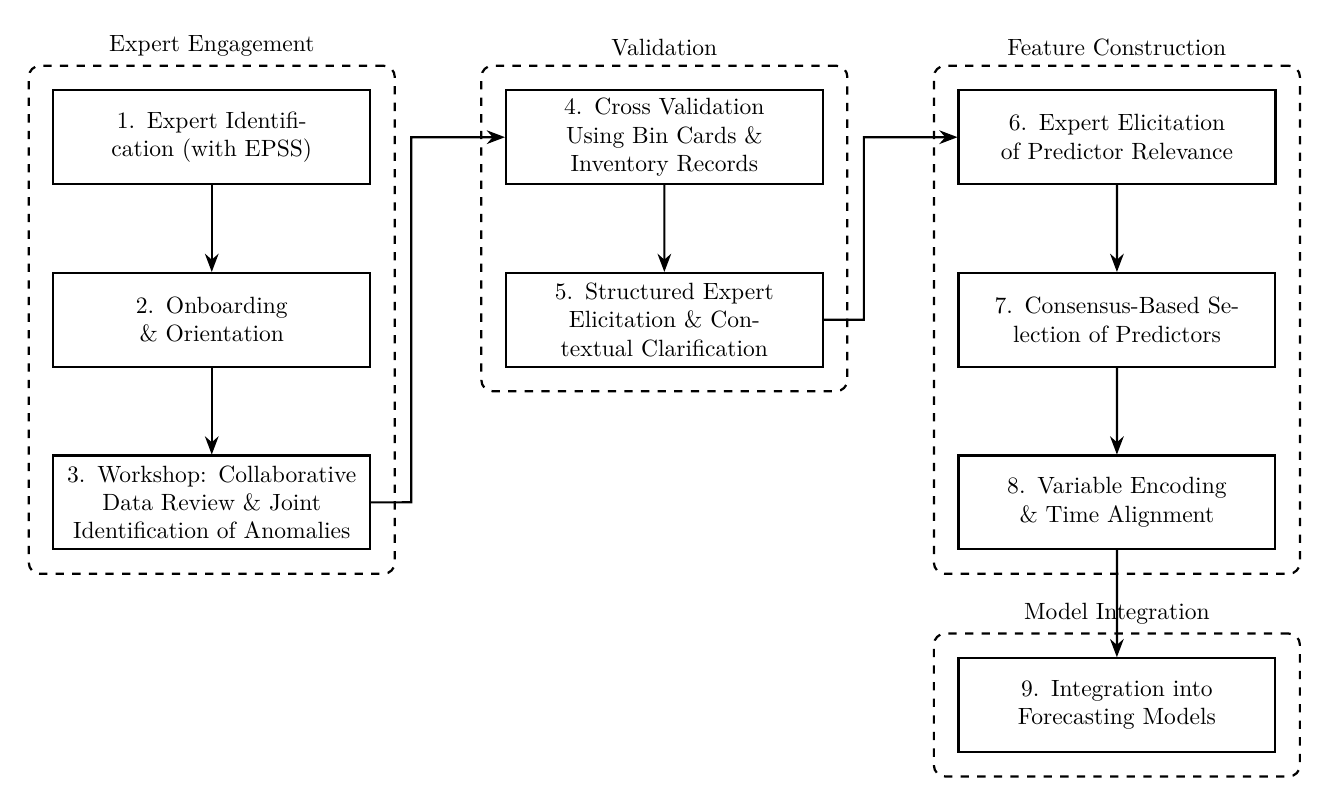
\begin{tikzpicture}[scale=0.85, transform shape, node distance=1.3cm and 2cm]

% Node style
\tikzset{
  process/.style={
    rectangle,
    draw=black,
    thick,
    text width=4.5cm,
    align=center,
    minimum height=1.4cm
  },
  arrow/.style={
    thick,
    ->,
    >=Stealth
  }
}

% Nodes
\node (step1) [process] {1. Expert Identification (with EPSS)};
\node (step2) [process, below=of step1] {2. Onboarding \& Orientation};
\node (step3) [process, below=of step2] {3. Workshop: Collaborative Data Review \& Joint Identification of Anomalies};

\node (step4) [process, right=of step1] {4. Cross Validation Using Bin Cards \& Inventory Records};
\node (step5) [process, below=of step4] {5. Structured Expert Elicitation \& Contextual Clarification};

\node (step6) [process, right=of step4] {6. Expert Elicitation of Predictor Relevance};
\node (step7) [process, below=of step6] {7. Consensus-Based Selection of Predictors};
\node (step8) [process, below=of step7] {8. Variable Encoding \& Time Alignment};

\node (step9) [process, below=of step8, yshift=-0.3cm] {9. Integration into Forecasting Models};

% Arrows
\draw [arrow] (step1) -- (step2);
\draw [arrow] (step2) -- (step3);

\path (step3.east) -- +(0.6,0) coordinate (s3stub);
\draw [arrow] (step3.east) -- (s3stub) |- (step4.west);

\draw [arrow] (step4) -- (step5);

\path (step5.east) -- +(0.6,0) coordinate (s5stub);
\draw [arrow] (step5.east) -- (s5stub) |- (step6.west);

\draw [arrow] (step6) -- (step7);
\draw [arrow] (step7) -- (step8);
\draw [arrow] (step8) -- (step9);

% Group boxes
\node[draw=black, thick, dashed, inner sep=0.3cm, rounded corners, fit=(step1)(step2)(step3), label={[black]90:Expert Engagement}] {};
\node[draw=black, thick, dashed, inner sep=0.3cm, rounded corners, fit=(step4)(step5), label={[black]90:Validation}] {};
\node[draw=black, thick, dashed, inner sep=0.3cm, rounded corners, fit=(step6)(step7)(step8), label={[black]90:Feature Construction}] {};
\node[draw=black, thick, dashed, inner sep=0.3cm, rounded corners, fit=(step9), label={[black]90:Model Integration}] {};

\end{tikzpicture}
\caption{Diagram illustrating the sequential steps involved in collecting, structuring, and utilizing domain knowledge for modeling.}
\label{fig:expert-pipeline}
\end{figure}

Through a facilitated half-day workshop, these experts reviewed five
years of monthly distribution data for 33 pharmaceutical products.
Anomalous patterns---such as distribution spikes, prolonged lows, and
erratic fluctuations---were jointly identified and interpreted in light
of operational events (e.g., emergency distributions, inventory cycles).
These insights were cross-validated against bin cards and warehouse
records, and internal transfers were excluded to isolate externally
relevant events. Dates were standardized to the Gregorian calendar.

Predictor variables were defined through expert consensus, with
inclusion contingent on agreement among all six core participants
regarding the operational relevance and causal validity of each factor.
The final predictors included binary indicators for stock replenishment
events, categorical variables for fiscal year inventory counts, and
dummy variables for malaria seasonality. A further description of these
variables is summarized as followings:

\begin{itemize}
\item
  Stock replenishment: refers to the process of restocking or refilling
  inventory to ensure that there are sufficient quantities of products
  or materials available to meet demand. Whenever there was stock
  replenishment at the central EPSS, distribution to hubs and health
  facilities increased. This increase was attributed to the need to
  restock depleted inventories and the push from central EPSS to manage
  space constraints.
\item
  Physical fiscal year inventory counting: refers to the process of
  manually counting and verifying the actual quantities of
  pharmaceutical products available in stock at a specific location. The
  process is critical for maintaining the accuracy of inventory records,
  ensuring that medicines are available when needed, and preventing
  stockouts or overstocking. Physical inventory counting periods also
  influenced distribution. Stores closed during these periods, halting
  transactions. We observed increased distribution before inventory
  counting periods, as hubs and facilities stocked up. July and August
  were identified as physical counting periods each year.
\item
  Malaria seasonality: refers to the predictable patterns and
  fluctuations in malaria incidence throughout the year, typically
  influenced by climate and environmental conditions. In many regions,
  malaria transmission peaks during and shortly after the rainy season,
  when conditions such as stagnant water pools create ideal breeding
  sites for the Anopheles mosquitoes that transmit the disease.
  Conversely, malaria cases often decline during the dry season when
  mosquito breeding sites are reduced. During peak malaria seasons,
  there is a significant surge in the demand for antimalarial drugs and
  other related treatments. Malaria seasonality was another significant
  predictor. Certain pharmaceuticals, like Artemether + Lumefanthrine
  and Rapid Diagnostic Test kits, were affected by malaria outbreaks. We
  identified two recurrent epidemic seasons each year---March to May and
  September to December---that affected distribution from 2017 through
  2022.
\end{itemize}

These predictors, encoded with known historical and future values, were
added to the modeling dataset. This approach ensured consistent
integration of expert-informed contextual variables across both point
and probabilistic forecasting models.

\subsection{Forecasting models}\label{forecasting-models}

We evaluate a range of univariate models and their counterparts that
include predictors, spanning from simpler methods like regression,
exponential smoothing, and ARIMA to more complex models such as long
short-term memory (LSTM) networks and advanced foundational time series
forecasting models. Below, we provide a brief overview of these
approaches. Detailed implementation codes in R and Python are available
in a GitHub repository and accessible for public.

\textbf{Exponential Smoothing State Space model (ETS):} ETS models, as
described by \citet{hyndman2021forecasting}, combine trend, seasonality,
and error components in time series using different configurations that
can be additive, multiplicative, or mixed. The trend component can be
specified as none (``N''), additive (``A''), or damped additive
(``Ad''); the seasonality can be none (``N''), additive (``A''), or
multiplicative (``M''); and the error term can be additive (``A'') or
multiplicative (``M''). To forecast distribution, we use the ETS()
function from the fable package in R, which automatically selects the
optimal model for each time series based on the corrected Akaike's
Information Criterion (AICc). In our study, an automated algorithm
determines the best configuration for trend, seasonality, and error
components across each time series, leveraging the ets() function's use
of AIC to identify the optimal model. Given the high volume of time
series (1530), manual selection of components is impractical, so the
algorithm customizes model forms for each series based on its unique
characteristics. This results in a tailored combination of additive or
multiplicative components, adapting to the specific patterns of each
time series.

\textbf{Multiple Linear Regression (MLR)}: We use Multiple linear
regression to model the relationship between a distribution and
potential variables influencing its variation. In our first model, we
use multiple linear regression with a trend component to capture the
underlying progression over time, i.e., \emph{regression}. We also
incorporate dummy variables for each month to account for seasonal
fluctuations, without including any additional predictors, i.e.,
\emph{regression\_reg}. This approach helps us establish a baseline
model focused solely on temporal trends and seasonal patterns. We then
extend this model by introducing additional predictors that include
variables such as replenishment cycles, fiscal year indicators, and
periods with malaria prevalence. These additional predictors allow the
model to see if capturing external factors can provide a better
understanding of the factors influencing the distribution and result at
enhanced accuracy. We produce forecasts using TLSM() function from the
fable package in R.

\textbf{ARIMA and ARIMA with regressors}: ARIMA (AutoRegressive
Integrated Moving Average) is a powerful statistical model designed to
forecast time series by capturing temporal dynamics and are widely used
in time series forecasting due to their ability to model complex trends
and patterns over time without relying on external predictors. ARIMAX
(Auto Regressive Integrated Moving Average with eXogenous variables)
extends ARIMA by incorporating external variables, or exogenous
predictors, into the model. This modification allows to include relevant
information from external factors such as malaria season, and fiscal
year period, and stock replenishement period that may explain variations
in the series beyond its internal time dynamics, we refer to this in the
result as \emph{arima\_reg}. By adding these predictors, ARIMAX combines
the strengths of ARIMA's time-series structure with the flexibility of
regression models. In our study, we use an automated algorithm to
determine the optimal configuration for ARIMA components, following the
approach outlined by \citet{hyndman2021forecasting} and We use the
ARIMA() function from the fable package in R.

\textbf{Long Short-Term Memory neural network (LSTM)}: The LSTM model is
a specialised form of recurrent neural network (RNN) used to model
sequential data by capturing long-term dependencies
\citep{graves2012long}. Unlike traditional RNNs, LSTMs can learn to
retain information for longer time periods due to their unique
architecture, which consists of several gates that control the flow of
information. This makes LSTMs particularly effective for time series
forecasting. In our implementation, we used a sequential model
architecture, comprising one LSTM layer with 50 units, followed by dense
layers, with the final output being a single linear unit. The Adam
optimizer was employed to minimize the mean squared error, and the model
was trained for 100 epochs using the keras\_model\_sequential() function
from the Keras package in R. We use LSTM models both with and without
predictors, referring to the LSTM model with predictors as
\emph{lstm\_reg}.

To improve the robustness of the LSTM models and address overfitting
issues, we introduced dropout regularization layers after the LSTM units
and employed early stopping based on validation loss during model
training. Each LSTM model was trained independently for each product
series. Hyperparameter tuning was performed in a preliminary phase using
a subset of products. Various configurations of LSTM units (30--100),
dense units (50--200), dropout rates (0.1--0.5), and batch sizes
(16--64) were evaluated based on validation set performance. The final
model structure --- 50 LSTM units, 100 dense units, a 0.2 dropout rate,
and a batch size of 32 --- was selected as a trade-off between forecast
accuracy and model stability across different demand patterns.

\textbf{TimeGPT}: TimeGPT is the first pre-trained foundational model
designed specifically for time series forecasting, developed by Nixtla
\citep{garza2023timegpt}. It uses a transformer-based architecture with
an encoder-decoder configuration but differs from other models in that
it is not based on large language models. Instead, it is built from the
ground up to handle time series data. TimeGPT was trained on more than
100 billion data points, drawing from publicly available time series
across various sectors, such as retail, healthcare, transportation,
demographics, energy, banking, and web traffic. This wide range of data
sources, each with unique temporal patterns, enables the model to manage
diverse time series characteristics effectively. Furthermore, TimeGPT
supports the inclusion of external regressors in its forecasts and can
generate quantile forecasts, providing reliable uncertainty estimation.
We use TimeGpt models both with and without predictors, referring to the
model with predictors as \emph{timegpt\_reg}.

\subsection{Generating probabilistic
forecasts}\label{generating-probabilistic-forecasts}

In addition to point forecasts, we generated probabilistic forecasts to
capture the uncertainty surrounding future pharmaceutical distribution
Several approaches are available for generating probabilistic forecasts,
including analytical prediction intervals, quantile regression, Bayesian
modeling through Markov Chain Monte Carlo (MCMC) methods, bootstrapping,
and conformal prediction \citep{wang2023}.

In this study, we employed a bootstrapping approach to construct
predictive intervals. Bootstrapping was chosen primarily for its
flexibility and model-agnostic nature, allowing it to be applied
uniformly across the diverse range of forecasting methods implemented
without requiring strong distributional assumptions. Moreover,
pharmaceutical distribution data often exhibit irregular and volatile
patterns, making non-parametric approaches like bootstrapping
particularly suitable.

Specifically, we assume that future forecast errors will be similar to
past forecast errors. The forecast error at time \(t\) is defined as:
\(e_t = y_t - \hat{y}_t\), where \(y_t\) represents the observed
distribution, and \(\hat{y}_t\) denotes the corresponding forecast
estimate. To simulate future distribution paths, we randomly sample
errors with replacement from the historical error distribution and add
them to the point forecast estimates. This process is repeated multiple
times (1,000 iterations in our study) to generate a distribution of
possible outcomes for each forecast horizon.

Prediction intervals at the desired confidence level (e.g., 95\%) are
then constructed by taking appropriate quantiles from the empirical
distribution of the simulated forecasts \citep{hyndman2021forecasting}.

The bootstrapping method thus provides a robust and flexible framework
to quantify forecast uncertainty across a heterogeneous set of
pharmaceutical products without imposing restrictive parametric
assumptions.

\subsection{Performance evaluation}\label{performance-evaluation}

To evaluate the performance of our forecasting models, we split the data
into a series of training and test sets and employed a time series
cross-validation approach, following best practices for forecasting
evaluation \citep{hyndman2021forecasting}. Rather than using a fixed
training and test split, we used a rolling-origin cross-validation
framework, which allows for a more comprehensive assessment across
different demand patterns and periods. In our setup, the initial
training set consisted of all available historical data from December
2017 up to June 2021. The evaluation period covered the subsequent 12
months, reflecting the operational needs of the EPSS, which plans
distribution over a one-year horizon. At each iteration, models were
trained on an expanding training window and evaluated over a fixed
6-month forecast horizon, aligned with typical EPSS planning cycles.
After each forecast generation, the training set was expanded by one
additional month, and the process was repeated, allowing for rolling
assessment across the final 12 months of data. This structure ensured
that forecasts reflected realistic operational scenarios, where
forecasts are continuously updated as new data becomes available. This
cross-validation design allowed us to evaluate each model's ability to
perform across multiple different forecast origins and a variety of
demand conditions, providing a more reliable and generalizable
understanding of model performance. Furthermore, all model development
steps, including hyperparameter tuning for the LSTM models, were
conducted exclusively using the training data available at each
iteration. No test set information was used during model selection or
tuning.

The error metrics presented here consider a forecasting horizon denoted
by by \(j\), which represents the number of time periods ahead we are
predicting, with \(j\) ranging from 1 to 6 months in our study. Point
forecast accuracy is measured using the Mean Squared Scaled Error (MSSE)
and the Mean Absolute Scaled Error (MASE). The Mean Absolute Scaled
Error (MASE) \citep{HK06, hyndman2021forecasting} is calculated as
follows:

\[
  \text{MASE} = \text{mean}(|q_{j}|),
\] where \[
  q_{j} = \frac{ e_{j}}
 {\displaystyle\frac{1}{T-m}\sum_{t=m+1}^T |y_{t}-y_{t-m}|},
\] and \(e_{j}\) is the point forecast error for forecast horizon \(j\),
\(m = 12\) (as we have monthly seasonal series), \(y_t\) is the
observation for period \(t\), and \(T\) is the sample size (the number
of observations used for training the forecasting model). The
denominator is the mean absolute error of the seasonal naive method in
the fitting sample of \(T\) observations and is used to scale the error.
Smaller MASE values suggest more accurate forecasts. Note that the
measure is scale-independent, thus allowing us to average the results
across series.

Here, \(e_{j}\) represents the point forecast error for forecast horizon
\(j\), with \(m = 12\) (since we are dealing with monthly seasonal
data). The term \(y_t\) denotes the observation at time \(t\), and \(T\)
is the sample size, or the number of observations used for training the
forecasting model. The denominator in the MASE formula is the mean
absolute error of the seasonal naive method over the training sample of
\(T\) observations, providing a basis for scaling the forecast error.
Lower MASE values indicate more accurate forecasts. Notably, this
measure is scale-independent, allowing us to average results across
different series for broader performance comparison.

A related measure is MSSE
\citep{hyndman2021forecasting, makridakis2022m5}, which uses squared
errors rather than absolute errors:
\begin{equation}\phantomsection\label{eq-RMSSE}{
  \text{MSSE} = \text{mean}(q_{j}^2),
}\end{equation} where, \[
  q^2_{j} = \frac{ e^2_{j}}
 {\displaystyle\frac{1}{T-m}\sum_{t=m+1}^T (y_{t}-y_{t-m})^2},
\] Again, this is scale-independent, and smaller MSSE values suggest
more accurate forecasts.

To measure the forecast distribution accuracy, we calculate the
Continuous Rank Probability Score (CRPS) \citep{hyndman2021forecasting}.
It rewards sharpness and penalizes miscalibration, so it measures
overall performance of the forecast distribution. For probabilistic
evaluation, 1,000 future paths were simulated per series, enabling
robust estimation of forecast uncertainty.

\begin{equation}\phantomsection\label{eq-CRPS}{
  \text{CRPS} = \text{mean}(p_j),
}\end{equation} where \[
  p_j = \int_{-\infty}^{\infty} \left(G_j(x) - F_j(x)\right)^2dx,
\] where \(G_j(x)\) is the forecasted probability distribution function
for forecast horizon \(j\), and \(F_j(x)\) is the true probability
distribution function for the same period.

Calibration refers to the statistical consistency between the
distributional forecasts and the observations. It measures how well the
predicted probabilities match the observations. On the other hand,
sharpness refers to the concentration of the forecast distributions ---
a sharp forecast distribution results in narrow prediction intervals,
indicating high confidence in the forecast. A model is well-calibrated
if the predicted probabilities match the distribution of the
observations, and it is sharp if it is confident in its predictions. The
CRPS rewards sharpness and calibration by assigning lower scores to
forecasts with sharper distributions, and to forecasts that are
well-calibrated. Thus, it is a metric that combines both sharpness and
miscalibration into a single score, making it a useful tool for
evaluating the performance of probabilistic forecasts.

CRPS can be considered an average of all possible quantiles
\citep[Section 5.9]{hyndman2021forecasting}, and thus provides an
evaluation of all possible prediction intervals or quantiles. A specific
prediction interval could be evaluated using a Winkler score, if
required.

\section{Results and discussion}\label{sec-results}

In this section, we compare the forecasting performance of various
approaches, examining models that incorporate expert-identified business
context predictors versus those that rely solely on historical
distribution data. Point forecast performance is reported using MASE and
RMSSE, while probabilistic forecast accuracy is reported using CRPS.

The forecasting performance is reported in Figure~\ref{fig-point}, in
which the average forecast accuracy over forecast horizon and across all
products is calculated for each origin. We report the distribution of
accuracy metrics across all rolling origins. This shows how models
varies in providing accuracy across different origins. The y-axis
displays models sorted by their MASE and RMSSE values, with the model
exhibiting the lowest error positioned at the bottom. This model is the
LSTM model, followed by ARIMA, which incorporate exogenous variables.
Additionally, Figure~\ref{fig-point} indicates that predictors obtained
through interactions with domain experts enhance point forecast accuracy
across most models. This underscores the critical importance of
systematically collecting such expert-informed data alongside
transactional distribution data.

\begin{figure}[H]

\centering{

\includegraphics{main_files/figure-pdf/fig-point-1.pdf}

}

\caption{\label{fig-point}Distribution of point forecast accuracy across
different origins, averaged across the forecat horizon and all products.
The total number of months used to calculate the accuracy in the test
set is 12 months for each product. MASE and MSSE are relative to the
corresponding values for the training set.}

\end{figure}%

\begin{figure}[H]

\centering{

\includegraphics{main_files/figure-pdf/fig-prob-1.pdf}

}

\caption{\label{fig-prob}Distribution of probabilistic forecast accuracy
across different origins, averaged across the forecat horizon and all
products. The total number of months used to calculate the accuracy in
the test set is 12 months for each product.}

\end{figure}%

Figure~\ref{fig-prob} illustrates the forecast distribution accuracy
measured by CRPS, which evaluates both forecasting calibration and
interval sharpness. A smaller CRPS value indicates better overall
performance. We observed that incorporating domain knowledge improved
forecast accuracy for most models, enhancing not only point forecasts
but also probabilistic forecasts. Notably, LSTM and ARIMA yielded the
most accurate probabilistic forecasts when identified predictors were
incorporated. This aligns with the findings related to point forecast
accuracy, reinforcing the earlier explanations for these results.

While LSTM models achieved the best overall forecast accuracy across
products, their performance exhibited notable variability depending on
the characteristics of individual demand patterns. For example, the
product \(Amlodipine - 5mg - Tablet\) demonstrates periods of extreme
variability, with spikes in demand followed by periods of very low or
zero distribution. Such patterns align well with the strengths of
univariate LSTM models, which are adept at capturing long-term
dependencies and managing complex temporal fluctuations. In contrast,
the demand for \(Anti-Rho (D)\) is erratic and sparse, with frequent
random fluctuations and little structural consistency. This lack of
clear temporal patterns can make it challenging for LSTM models to learn
generalizable signals, particularly given the limited data length
available for training. Although LSTM can manage irregular data to some
extent, it performs best when patterns are consistent or cyclic. These
variations across product types contributed to the observed distribution
of forecast errors across the product portfolio. Moreover, although we
expect that multivariate LSTM models benefit from expert-informed
predictors, our results show that the univariate LSTM consistently
achieved better forecast performance. This outcome may be attributed to
the nature of the predictors---binary, static, or weakly aligned with
short-term temporal dynamics---which can disrupt rather than enhance
learning when added to a neural network sensitive to input
configuration. Moreover, with relatively short historical series and
limited training samples, the inclusion of additional variables may have
led to overfitting or reduced generalization. These findings suggest
that while LSTM models can effectively learn temporal patterns from
distribution data alone, incorporating structured external knowledge
requires careful feature engineering and alignment to be beneficial.

The findings emphasize the importance of incorporating relevant domain
knowledge into forecasting models. In pharmaceutical supply logistics
administration systems, data often consists solely of transactional
records on distribution and distribution. Including exogenous variables
such as administrative procedures, seasonal patterns, or conflicts, or
any other relevant factor that could be identified by those with domain
knowledge proved essential for reducing forecast errors. This approach
improved both point and probabilistic forecast accuracy, enabling a more
confident assessment of uncertainty. Therefore, the systematic
collection of information about significant events and their impact on
distribution is vital. Recording details of events such as policy
changes, administration procedures, conflicts, and incorporating this
information into forecasting models creates a comprehensive
understanding of distribution. This practice enhances modeling
reliability and allows institutions in developing countries and
humanitarian organizations to better forecast demand, allocate resources
effectively, and respond proactively. Establishing robust data
collection systems is thus a critical step for strengthening forecasting
capabilities and operational resilience.

\subsection{Computational efficiency and resource
considerations}\label{computational-efficiency-and-resource-considerations}

In addition to forecast accuracy, it is also important to consider the
computational efficiency of each model, particularly in settings where
computational resources and technical expertise are limited.

Table~\ref{tbl-runtime} shows the total runtime required to train and
generate forecasts across all 33 pharmaceutical product time series for
each method for all origins. All models were implemented using R, except
TimeGPT, which was run via Google Colab using a T4 GPU backend. All
other models were executed on a local machine with 7 CPU cores (11th Gen
Intel(R) Core(TM) i5-1135G7 @ 2.40 GHz and 8 GB RAM)

\begin{table}[H]

\caption{\label{tbl-runtime}Computation time required for training and
generating forecasts for each model across all products.}

\centering{

\centering\begingroup\fontsize{11}{13}\selectfont

\begin{tabular}{lrll}
\toprule
Model & Runtime (Seconds) & Runtime type & category\\
\midrule
\cellcolor{gray!6}{LSTM} & \cellcolor{gray!6}{6892.30} & \cellcolor{gray!6}{CPU with 7 cores} & \cellcolor{gray!6}{high}\\
LSTM with regressors & 7234.00 & CPU with 7 cores & high\\
\cellcolor{gray!6}{Regression} & \cellcolor{gray!6}{27.48} & \cellcolor{gray!6}{CPU with 7 cores} & \cellcolor{gray!6}{low}\\
Regression with regressors & 47.38 & CPU with 7 cores & low\\
\cellcolor{gray!6}{ARIMA} & \cellcolor{gray!6}{96.27} & \cellcolor{gray!6}{CPU with 7 cores} & \cellcolor{gray!6}{low}\\
ARIMA with regressors & 138.08 & CPU with 7 cores & medium\\
\cellcolor{gray!6}{TimeGPT} & \cellcolor{gray!6}{2.57} & \cellcolor{gray!6}{Colab T4 GPU} & \cellcolor{gray!6}{low}\\
TimeGPT with regressors & 3.72 & Colab T4 GPU & low\\
\cellcolor{gray!6}{ETS} & \cellcolor{gray!6}{75.71} & \cellcolor{gray!6}{CPU with 7 cores} & \cellcolor{gray!6}{low}\\
\bottomrule
\end{tabular}
\endgroup{}

}

\end{table}%

As shown in Figure 4 and 5, models that incorporated expert-informed
regressors generally achieved better forecast accuracy compared to their
univariate versions. This trend was most evident in classical models
such as ARIMA and regression, where the inclusion of regressors led to a
noticeable shift toward lower and more concentrated error distributions.
However, this improvement came with an increase in computational cost.
In all cases, the addition of regressors increased runtime---by 72\% in
the regression model (from 27.48 to 47.38 seconds) and by 43\% in ARIMA
(from 96.27 to 138.08 seconds). TimeGPT also showed a slight increase in
runtime (from 2.57 to 3.72 seconds), although the total processing time
remained extremely low overall. Moreover, LSTM exhibited the largest
increase in runtime when regressors were added, rising from 6,892 to
7,234 seconds. This sharp increase reflects the sensitivity of neural
networks to input configuration, especially in contexts with limited
data, irregular demand, and noisy signals.

These results underscore the importance of balancing model performance
with implementation cost. While deep learning models such as LSTM offer
strong potential when well-tuned, they demand significantly more
computational resources and may be less robust when integrating static
or weakly aligned contextual features. By contrast, TimeGPT, a
foundational model pretrained on large-scale time series data, provides
a compelling alternative. It required less than 4 seconds to forecast
all products, offered competitive accuracy, and required no tuning or
retraining---making it well-suited for practical use in low-resource
environments.

\subsection{An illustration of probabilistic forecast for Pharmaceutical
product
distribution}\label{an-illustration-of-probabilistic-forecast-for-pharmaceutical-product-distribution}

In this section, we present an illustrative example of a probabilistic
forecast for future distribution of \emph{Sodium Chloride (Normal
Saline)} product. Due to the complexity of including such visualizations
for all products, only one example is shown here. However, it is
feasible to generate these plots for all products if needed.

In practice, point forecasts are commonly used despite their
limitations, but they do not account for the inherent uncertainty
associated with forecasts. The future is inherently uncertain, and
effective planning requires considering alternative scenarios.
Probabilistic forecasts offer a comprehensive approach by assigning
likelihoods to a range of possible outcomes, recognizing that different
distribution levels may occur with varying probabilities. The goal is to
maximize the sharpness of these predictive distributions---i.e., how
concentrated the forecasts are---while maintaining calibration, meaning
that the predicted probabilities align well with actual outcomes
\citep{gneiting2014probabilistic}. This approach allows decision-makers
to fully leverage available information, incorporating uncertainty in a
structured and measurable way. The primary purpose, as illustrated in
Figure~\ref{fig-forecast-density-hstep}, is to quantify and communicate
uncertainty. This figure displays the forecast distribution of
distribution over a 6-month horizon using a density plot. For each month
within the forecast period, a separate distribution is generated. The
plot also includes the point forecast alongside 80\% and 90\% prediction
intervals to illustrate potential variability.

Probabilistic forecasts enhance planning and decision-making by offering
a comprehensive view of potential future outcomes and their likelihood,
rather than relying on a single point estimate. A probabilistic forecast
takes the form of a predictive probability distribution over future
quantities or events of interest.

It is important to note that while point forecasts and prediction
intervals can be derived from probabilistic forecasts, the reverse is
not true. A single-point forecast cannot inherently provide the
probabilistic context needed to capture the range of possible outcomes.
Although prediction intervals can indicate a range of potential values,
they do not convey the detailed probabilities of low or high
distribution. This distinction highlights the value of probabilistic
forecasting in supporting informed decision-making by offering a clearer
view of future uncertainties.

\begin{figure}[H]

\centering{

\includegraphics{main_files/figure-pdf/fig-forecast-density-hstep-1.pdf}

}

\caption{\label{fig-forecast-density-hstep}A graphical illustration of
the forecast distribution of a pharmacutical product (i.e.~total
incidence attended) for the SB health board for a horizon of six month.
For each month, we display the point forecast (black point), the
histogram, and 80\% (thick line) and 90\% (thin line) prediction
intervals. It also shows a portion of a historical time series as well
as its fitted values.}

\end{figure}%

To further illustrate the practical relevance, we consider an
illustrative case where the mean forecasted distribution for the next
month is 1,000 units, with a 90\% prediction interval ranging from 850
to 1,150 units. Table~\ref{tbl-point_vs_probabilistic} summarizes the
decision outcomes under each approach.

Under a traditional approach, inventory decisions would rely solely on
the point forecast. Based on the mean prediction of 1,000 units, the
store manager would order precisely that quantity, assuming it would
meet the expected demand. However, this approach does not incorporate
any adjustment for uncertainty, potentially leading to stockouts if
actual demand exceeds 1,000 units, or excess inventory if distribution
is lower.

In contrast, utilizing the full probabilistic forecast allows the
decision-maker to take variability into account. If a higher service
level is required, for example 95\%, the inventory policy may be
adjusted by stocking closer to the upper bound of the 90\% prediction
interval (e.g., 1,150 units). If inventory holding costs are a major
concern and the organization can tolerate a modest risk of shortage, the
order quantity could remain closer to the median forecast of 1,000
units.

\begin{table}[H]

\caption{\label{tbl-point_vs_probabilistic}Comparison of ordering
decisions under point and probabilistic forecasts - an illustrative
example.}

\centering{

\centering\begingroup\fontsize{11}{13}\selectfont

\resizebox{\linewidth}{!}{
\begin{tabular}{lll}
\toprule
Forecast Type & Ordering Quantity & Risk Consideration\\
\midrule
Point Forecast Only & 1,000 units & No explicit consideration of uncertainty\\
Probabilistic Forecast (95\% service level) & 1,150 units & Adjusts inventory to account for demand variability\\
\bottomrule
\end{tabular}}
\endgroup{}

}

\end{table}%

This illustrative comparison indicates that point forecasts provide a
single estimate without adjusting for forecast uncertainty, while
probabilistic forecasts allow decision-makers to explicitly align
inventory decisions with risk tolerance and service level requirements.
This is particularly important for pharmaceutical products, where the
consequences of stockouts or overstocking can be significant both
operationally and clinically.

\subsection{Managerial Implications}\label{managerial-implications}

This study offers actionable lessons for supply chain managers, public
health planners, and policymakers navigating the uncertainty of
pharmaceutical demand---particularly in systems like Ethiopia, where
operational constraints and demand volatility are the norm, not the
exception.

At present, national forecasting at the EPSS still relies heavily on
basic extrapolation tools---usually Excel sheets or donor-developed
software such as the Quantification Analysis Tool (QAT). These tools are
easy to use but limited: they assume stable demand, ignore uncertainty,
and often miss the operational signals embedded in local experience. In
practice, forecasts are sometimes adjusted based on gut feeling or
anecdotal program insights---not because planners want to---but because
the tools don't offer a better alternative.

The models developed here---freely available, open-source, and designed
to integrate directly with routine EPSS data---allow planners to make
decisions using full probabilistic forecasts, not just single-point
estimates. Forecasts are delivered with prediction intervals (e.g., 80\%
or 90\%) that help teams decide not only how much to order, but how much
risk they're willing to tolerate. For products with known
seasonality---like antimalarials or diagnostic kits---this matters. The
system doesn't just forecast a number; it gives planners a buffer
strategy.

Beyond accuracy, the models also reflect how medicines actually move
through the system. Predictors based on warehouse replenishments, fiscal
year inventory routines, and known disease cycles are embedded into the
forecasts---not hard-coded, but learned from the data in ways that are
transparent and reproducible. These inputs are drawn from expert
operational knowledge and can be updated or modified as the system
evolves.

Importantly, the entire modeling pipeline is built in R and Python, and
is already shared alongside code and data. This makes it immediately
usable by EPSS analysts and regional logistics teams, even in settings
without access to proprietary tools or high-end infrastructure. It's not
a black box; it's something the system can own, modify, and grow with.

To support real uptake, we recommend five practical steps:

\begin{itemize}
\item
  Embed these probabilistic models into EPSS quantification rounds to
  replace rigid extrapolation methods and bring scenario-based planning
  into monthly and quarterly cycles.
\item
  Use prediction intervals to define risk-informed buffer policies,
  especially for high-volatility products. Not every item needs the same
  margin of error.
\item
  Automate the collection of domain knowledge (e.g., replenishment
  events, stock counts, seasonal triggers) into the logistics data
  stream to reduce reliance on manual elicitation while preserving
  contextual intelligence.
\item
  Train regional and central teams using the open-source tools and
  shared codebase, turning forecasting into a hands-on, in-country
  competency rather than a dependency on external tools or consultants.
\item
  Establish routine forecast review sessions, supported by visual
  dashboards that reflect not just what the model says, but how
  uncertain that estimate is---and what that means for stock levels,
  procurement plans, and emergency readiness.
\end{itemize}

Taken together, these steps push forecasting beyond formulas and into
real decision-making. For immediate short-term adoption in EPSS,
automating the integration of domain knowledge into logistics data
streams is critical to improve data quality and reduce manual efforts.
Establishing routine forecast review sessions supported by visual
dashboards can also be implemented in the short term to increase
transparency and incorporate uncertainty into decision-making. Following
these steps, embedding probabilistic forecasting methods and using
prediction intervals to design risk-informed buffer policies will
enhance planning accuracy and inventory resilience. Finally, training
regional and central teams using open-source tools should be pursued as
a long-term goal to build sustainable, in-country forecasting expertise.

\section{Conclusion and future research}\label{sec-conclusion}

In this study, we conducted an extensive analysis of pharmaceutical
demand forecasting within the EPSS. Using five years of distribution
data for 33 key pharmaceutical products, along with additional
information gathered through collaboration with domain experts at EPSS,
our goal is to enhance the demand forecasting process and emphasize the
importance of integrating domain knowledge into model building. This
step is critical, as the phase of understanding the data and
incorporating valuable contextual information is often overlooked. Too
frequently, forecasting efforts rely solely on distribution data,
leading to building models with little relevance to reality. Our
approach highlights the necessity of including domain insights to
construct more accurate and effective forecasting models.

Our findings highlight the importance of collecting and incorporating
domain knowledge when building forecasting models. We evaluated both
point and probabilistic forecasts using a range of models, from simple
univariate approaches like ARIMA to complex models such as LSTM. We
demonstrated that while the use of complex models may improve forecast
accuracy in the pharmaceutical supply context, this comes at the cost of
significantly increased computational time---an important consideration
for resource-constrained settings in low- and middle-income countries
(LMICs). Additionally, our research indicates that newly developed
foundational time series forecasting models hold promise, particularly
in settings with limited computational infrastructure and constrained
access to advanced analytical expertise, as often seen in pharmaceutical
supply chains in developing countries.

To advance forecasting practices further, exploring additional predictor
variables---such as public health campaigns, disease outbreaks, and
economic indicators---could provide valuable insights into demand
dynamics. Improving the granularity of historical distribution data,
through finer temporal intervals and geographic differentiation, also
holds potential for more precise predictions. Additionally, hybrid
forecasting models that combine judgmental point forecasts with
probabilistic machine learning models could enhance predictive
performance. Empowering EPSS staff through training in foundation models
for time series analysis and forecasting, data interpretation, and
collection will enable informed decision-making and strengthen workforce
capabilities. Replicating this study across diverse healthcare settings
and conducting comparative analyses would help validate the adaptability
and applicability of the findings. Additionally, it is recommended that
pharmaceutical supply services systematically collect and maintain
detailed records of events that may influence distribution, alongside
past distribution data. This practice is essential for refining demand
models and enhancing forecast accuracy.

\subsection{Practical challenges and
limitations}\label{practical-challenges-and-limitations}

Despite dedicated efforts to engage with domain experts to better
understand the data---and spending significant time over two weeks
collaborating with them---we found that the process of interpreting data
through domain knowledge is complex and presents unique challenges.
These challenges include defining what constitutes domain knowledge and
determining how best to incorporate it to enhance model reliability and
accuracy. Below, we summarize some of these key challenges. One issue
involved capturing accurate information from bin cards and expert
review, particularly during periods of disruption like COVID-19 and
conflicts. For instance, during the COVID-19 pandemic, experts noted a
decrease in demand due to travel restrictions. However, despite the
reduced demand, there were still significant distributions of
pharmaceuticals from the EPSS central to various hubs and health
facilities. This was because, in response to anticipated shortages, a
political decision was made to push products to these facilities before
the travel restrictions took full effect. The rationale was that if the
facilities remained closed, patients would have no access to
medications, necessitating the preemptive stockpiling of essential
pharmaceuticals. This scenario illustrates how policy decisions can
significantly impact supply chain data, making it challenging to model
distribution patterns accurately. Similarly, experts indicated that
conflicts would disrupt the distribution of pharmaceuticals. While
conflict zones did indeed hinder transportation, distribution still
occurred whenever roads were temporarily opened, even amidst ongoing
conflict. This created inconsistencies in the data, as periods of halted
distribution were followed by rapid replenishment once access was
restored. Such fluctuations add complexity to modelling the supply chain
from the central EPSS to hubs and health facilities. Other challenges
involved seasonal or periodic activities, such as the fiscal year-end
stock counting. During this time, EPSS temporarily halts transactions to
conduct a full inventory count, which can take anywhere from one to two
months, depending on the circumstances. This inconsistency in the
duration of inventory counts adds a layer of unpredictability to supply
chain modelling.

\subsection{Future research}\label{future-research}

Following the current research, several promising areas could further
advance knowledge and practical applications in this area:

\begin{itemize}
\item
  Future research could focus on developing intelligent systems that
  incorporate domain-specific knowledge into model building. This would
  involve creating algorithms capable of identifying relevant domain
  insights and integrating them effectively into model training
  processes. Such tools would bridge the gap between purely data-driven
  approaches and expert-knowledge-enhanced modeling, leading to more
  robust and contextually informed forecasts.
\item
  Large Language Models (LLMs) for time series forecasting, like the one
  included in this study, offer transformative opportunities for
  developing countries by making advanced forecasting methods
  accessible, even in contexts with limited expertise or infrastructure.
  However, future research should explore their applicability,
  advantages, limitations, and performance relative to traditional and
  hybrid forecasting methods.
\item
  Disruptions such as the COVID-19 pandemic and armed conflicts may
  alter distribution patterns in time series data, introducing
  irregularities that challenge the assumptions of traditional
  forecasting methods. In such contexts, it becomes important not only
  to model observed distribution but also to account for censored
  demand---i.e., the unmet need that would have been fulfilled under
  normal conditions and is essential for effective replenishment
  planning. Future research could focus on developing and evaluating
  forecasting strategies that are specifically designed to handle
  disrupted time series and estimate censored demand. In particular,
  methods that enhance the robustness of probabilistic forecasts in the
  presence of structural breaks or exogenous shocks are especially
  relevant. One promising direction is also the development of causal
  forecasting models that incorporate policy changes, epidemic dynamics,
  and socio-economic factors---an approach that may be particularly well
  suited to the realities of pharmaceutical supply chains in low- and
  middle-income countries (LMICs).
\item
  Future research should explore the integration of probabilistic
  forecasting into inventory management policies, with a focus on
  evaluating the operational impact of forecast uncertainty. In
  addition, there is substantial potential in leveraging more granular
  data---such as daily or weekly distribution patterns---and examining
  forecasts at hierarchical levels, including individual sites or health
  facilities. Investigating how fine-grained temporal and spatial
  forecasts influence decision-making in inventory control could provide
  valuable insights into reducing stockouts, minimizing holding costs,
  and decreasing pharmaceutical waste.
\end{itemize}

\section*{Reproducibility}\label{reproducibility}
\addcontentsline{toc}{section}{Reproducibility}

To enhance transparency and reproducibility, we not only provide data
and the code, but also the entire paper that is written in R \& Python.
All materials to reproduce this paper is available at
\href{https://github.com/arebuissa/Forecasting_EPSS_domain_knowledge}{this
Github repository}.

The repository contains the raw data, all R and Python scripts used in
experiments, the results used in the paper, as well as the quarto files
for producing this paper.


\renewcommand\refname{References}
  \bibliography{references.bib}


\end{document}
